\documentclass{article}

% if you need to pass options to natbib, use, e.g.:
%     \PassOptionsToPackage{numbers, compress}{natbib}
% before loading neurips_2021

% ready for submission
\usepackage[final]{neurips_2021}

% to compile a preprint version, e.g., for submission to arXiv, add add the
% [preprint] option:
%     \usepackage[preprint]{neurips_2021}

% to compile a camera-ready version, add the [final] option, e.g.:
%     \usepackage[final]{neurips_2021}

% to avoid loading the natbib package, add option nonatbib:
%    \usepackage[nonatbib]{neurips_2021}

\usepackage[utf8]{inputenc} % allow utf-8 input
\usepackage[T1]{fontenc}    % use 8-bit T1 fonts
\usepackage{hyperref}       % hyperlinks
\usepackage{url}            % simple URL typesetting
\usepackage{booktabs}       % professional-quality tables
\usepackage{amsfonts}       % blackboard math symbols
\usepackage{nicefrac}       % compact symbols for 1/2, etc.
\usepackage{microtype}      % microtypography
\usepackage{xcolor}         % colors
\usepackage{amsmath}
\usepackage{verbatim}
\usepackage[mathscr]{euscript}
\usepackage{graphicx}
\title{Machine Learning, 2024 Spring\\Assignment 4}
% The \author macro works with any number of authors. There are two commands
% used to separate the names and addresses of multiple authors: \And and \AND.
%
% Using \And between authors leaves it to LaTeX to determine where to break the
% lines. Using \AND forces a line break at that point. So, if LaTeX puts 3 of 4
% authors names on the first line, and the last on the second line, try using
% \AND instead of \And before the third author name.



\begin{document}

\maketitle

\begin{abstract}

\end{abstract}

\textcolor{blue}{Problem 1}
For problem 3 in assignment 3, change your GD code to SGD and complete the tasks below:
\begin{itemize}
	\item Present your code.
    \item How to choose (mini -) batch size?
    \item How to choose learning rate?
    \item How to terminate?
    \item Demonstrate the impact of different learning rates on the accuracy of the solution. In other words, your program should  output an image similar to the image on page 34 of the Lecture 6-SGD PPT.
\end{itemize}

\textcolor{blue}{Solution:}\\
0. Data preparation: The data is the same as the data in assignment 3.:
The data is divided into training set and validation set. The training set is used to train the model, and the validation set is used to evaluate the model. The data is normalized to make the data have zero mean and unit variance. The data is shuffled to make the data have no order.

1. The code and the method to run the code are all in the folder `code'.

2. The mini-batch size is set to be $1$ as we are applying the stochastic gradient descent.

3. The learning rate $\eta$ is tried with the following values: $0.1, 0.01, 0.001, 0.0001$. The learning rate for each step is similarly with the GD method, i.e. set $\eta_t = \eta\|\nabla e_t\|$. The learning rate is chosen by the learning rate schedule. 
From the results show in Figure \ref{fig:learning_rate}, we can see that the learning rate $\eta = 0.1$ is too large, which makes the loss diverge. The learning rate $\eta = 0.01$ is also too large, which makes the loss oscillate.
The learning rate $\eta = 0.001$ is a good choice, which makes the loss converge. The learning rate $\eta = 0.0001$ is too small, which makes the loss converge slowly.
So we finally choose the learning rate $\eta = 0.001$.
The accuracy in the validation set.



4. The termination condition is chosen by the number of iterations. The number of iterations should be large enough to make the loss converge.

5. The impact of different learning rates on the accuracy of the solution is shown in Figure \ref{fig:learning_rate}.

% \begin{figure}[htbp]
%   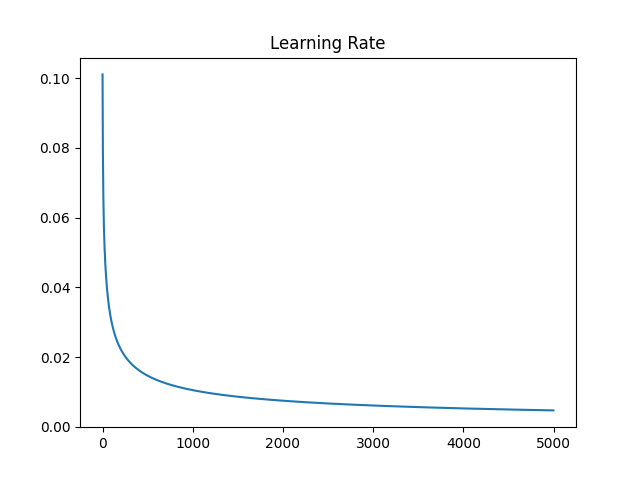
\includegraphics[width=0.5\textwidth]{../image/learning_rate.png}
%   \caption{Impact of different learning rates on the accuracy of the solution}
% \label{fig:learning_rate}
% \end{figure}














\end{document}